\chapter{Lecture 1: Topics in String Theory}

These notes follow Leonard Susskind's first lecture in the supplementary track on cosmology and black holes. The lecture begins with a philosophical challenge to reductionism, then turns that challenge into mathematics by way of bosonization, electric--magnetic duality, D-branes, strong coupling, emergent dimensions, and finally the combinatorial landscape of string vacua. The goal of this first-pass draft is to preserve the lecture's order of motivation while giving the mathematical backbone a cleaner written form. Notes curated by LazyingArt LLC.

\section{Reductionism and the Failure of Simplicity}

Susskind opens with the familiar picture that big things are made of little things, and that as one goes deeper one should eventually arrive at smaller and simpler building blocks. His deliberately ordinary metaphor is that houses are made of bricks, and nobody confuses the house with the brick: the brick is smaller and also simpler. The lecture begins by asking whether elementary particle physics actually behaves that way.

His first move is quantitative. The complaint is not yet about duality or string theory; it is that modern particle physics does not look especially simple even before quantum gravity enters. In the lecture these numbers are rough counts, but the roughness is part of the point:
\begin{equation}
N_{\mathrm{species}} \sim 75,
\qquad
N_{\mathrm{independent}} \sim 10\text{--}20,
\qquad
N_{\mathrm{parameters}} \sim 20.
\end{equation}
The Standard Model, however, is incomplete: gravity is absent, dark matter is absent, inflationary ingredients are absent, and the hierarchy problem pushes one toward additional structure. In the lecture Susskind uses supersymmetry as the clean example of what happens next: the theory becomes less, not more, economical. Schematically,
\begin{equation}
N_{\mathrm{parameters}}^{\mathrm{extended}} \sim 200.
\end{equation}

The force of this opening is rhetorical but precise. If reductionism were delivering increasing simplicity in the naive ``houses and bricks'' sense, then by this point one might have expected a short list of particles and a short list of constants. Instead one finds a theory with many moving parts, and that motivates the sharper question that governs the rest of the lecture:

\begin{remark}
The real issue is not merely that the current low-energy theory is complicated. The deeper question is whether there is even a unique, coupling-independent distinction between the basic objects and the composite ones.
\end{remark}

\section{Bosonization and the Loss of Fixed Fundamentality}

Susskind's first technical example is intentionally simple: a quantum field theory in one spatial dimension and one time dimension. He does not derive the equivalence in detail, and these notes will follow that choice. The point of the example is structural.

One starts with a field theory of fermions. The fermion field is denoted by \(\psi\). Two nearby fermions can form a bosonic composite, and the bosonic field that creates such composites is denoted by \(\phi\). At first sight the hierarchy seems clear: \(\psi\) is fundamental and \(\phi\) is effective.

The surprise is that the same theory can be rewritten the other way around, with the bosonic field \(\phi\) taken as the starting point. In that bosonic language the fermion is no longer represented as a point-like constituent but as a solitonic configuration, a kink in \(\phi\). The minimal mathematical content of the lecture is the interpolation itself:
\begin{equation}
\phi(x\to -\infty)=\phi_-,
\qquad
\phi(x\to +\infty)=\phi_+.
\end{equation}
A convenient schematic profile, used here only to make the spoken picture explicit, is
\begin{equation}
\phi(x)\approx \frac{\phi_++\phi_-}{2}
+
\frac{\phi_+-\phi_-}{2}\tanh\!\left(\frac{x}{\ell}\right).
\end{equation}
This is not meant to import a full sine-Gordon/Thirring derivation into the lecture. It is only a clean way to record Susskind's spoken description of a field that changes smoothly from one asymptotic value to another over some finite width \(\ell\).

The belt analogy in the lecture is mathematically apt. A belt with no twist represents a configuration without a kink. A belt whose orientation has rotated by \(2\pi\) between two distant points returns to the same local appearance at either end, but it must interpolate through a twisted region in between. That extended twisted region is the kink.

The role of the coupling \(G\) is then the essential point. Susskind emphasizes not an abstract equivalence but a coupling-dependent economy of description:
\begin{align}
G\ll 1
&\Rightarrow
\ell \text{ small, the kink is tight, and the }\psi\text{-description is efficient},\\
G\gg 1
&\Rightarrow
\ell \text{ large, the kink spreads out, and the }\phi\text{-description is efficient}.
\end{align}

\paragraph{A schematic update rule.}
\begin{enumerate}
\item Start with the fermionic description \(\psi\), where the bosons look like composites.
\item Rewrite the same theory in bosonic variables \(\phi\).
\item In that description the fermion appears as a kink of width \(\ell\).
\item For small \(G\), the kink is tight and the fermion looks elementary.
\item Increase \(G\), and the kink spreads out.
\item As the kink spreads, the bosonic variables become the simpler variables.
\end{enumerate}

This is the first place in the lecture where the question ``which are the bricks and which are the houses?'' stops having a unique answer.

\section{Weak and Strong Coupling in Quantum Electrodynamics}

The lecture next asks whether a similar reversal happens in more familiar particle physics. The example is electric charge versus magnetic monopole. The electron is the model electric monopole: an ordinary charged particle surrounded by an electric field. Susskind introduces the fine-structure constant \(\alpha\) as the relevant dimensionless strength parameter, and speaks of it heuristically as the square of the electric charge:
\begin{equation}
\alpha \sim e^2,
\qquad
\alpha \approx 10^{-2}
\quad
\text{in the lecture's rough ``about \(1/100\)'' estimate.}
\end{equation}
This is not intended as a precision convention; it is the lecture's way of tying \(\alpha\) to the probability for radiative processes.

When \(\alpha\) is small, the electron is simple: the surrounding electric field is weak, vacuum polarization is mild, and the particle looks nearly point-like. The magnetic monopole, by contrast, is then a strongly interacting, broad, heavy object. Susskind's weak--strong comparison can be summarized as
\begin{align}
\alpha \ll 1
&\Rightarrow
\text{electron simple, monopole heavy and extended},\\
\alpha \gg 1
&\Rightarrow
\text{monopole simple, electron heavy and structured}.
\end{align}
The lecture's emphasis is not on a detailed mass formula but on a reversal of descriptive convenience. At weak electric coupling one naturally builds QED from electrons, not monopoles. If one could dial the coupling past \(\alpha\sim 1\), the convenient language would exchange.

\begin{figure}[h]
\centering

\includegraphics[width=0.72\textwidth]{lecture_01_figure_02.png}

\vspace{1em}

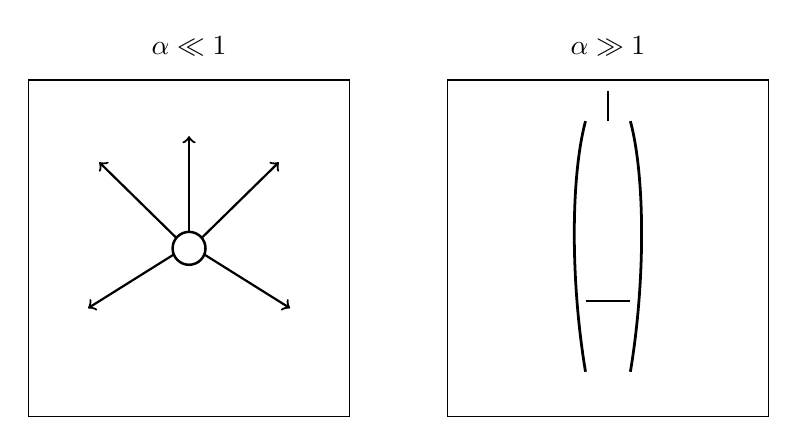
\begin{tikzpicture}[scale=0.95]
\draw (-5.3,-2.4) rectangle (-1.0,2.1);
\draw (0.3,-2.4) rectangle (4.6,2.1);

\node at (-3.15,2.55) {$\alpha \ll 1$};
\node at (2.45,2.55) {$\alpha \gg 1$};

\draw[line width=0.9pt] (-3.15,-0.15) circle (0.22);
\draw[->,line width=0.8pt] (-3.15,0.07) -- (-3.15,1.35);
\draw[->,line width=0.8pt] (-2.98,-0.01) -- (-1.95,1.00);
\draw[->,line width=0.8pt] (-3.32,-0.01) -- (-4.35,1.00);
\draw[->,line width=0.8pt] (-2.95,-0.23) -- (-1.80,-0.95);
\draw[->,line width=0.8pt] (-3.35,-0.23) -- (-4.50,-0.95);

\draw[line width=1.0pt] (2.15,-1.8) .. controls (1.95,-0.6) and (1.95,0.8) .. (2.15,1.55);
\draw[line width=1.0pt] (2.75,-1.8) .. controls (2.95,-0.6) and (2.95,0.8) .. (2.75,1.55);
\draw[line width=0.8pt] (2.15,-0.85) -- (2.75,-0.85);
\draw[line width=0.8pt] (2.45,1.55) -- (2.45,1.95);
\end{tikzpicture}
\caption{Susskind's blackboard comparison between \(\alpha\ll 1\) and \(\alpha\gg 1\). The screenshot is kept as visual evidence for the board layout; the redraw preserves only the transcript-backed contrast between a compact simple object and an extended heavy one.}
\end{figure}

A student question then lets Susskind recast the same point in ordinary QED language. One draws an electron worldline, lets it emit photons, then lets those photons create electron--positron pairs, and then lets the daughter charged lines radiate again. The lecture's claim is that there is no final smooth point-particle picture waiting at the end of that hierarchy; quantum fields fluctuate on every scale.

\begin{figure}[h]
\centering
\begin{tikzpicture}[scale=1.0]
\draw[->] (-1.2,0) -- (3.6,0) node[right] {space};
\draw[->] (0,-0.2) -- (0,4.3) node[above] {time};

\draw[line width=0.9pt] (0,0.2) -- (0,4.0);
\node[left] at (0,3.6) {\(\,e^{-}\)};

\draw[line width=0.8pt] (0,1.0) -- (0.18,1.08) -- (0.36,0.92) -- (0.54,1.10) -- (0.72,0.94) -- (0.90,1.12) -- (1.08,0.96) -- (1.26,1.14);
\draw[line width=0.8pt] (0,2.35) -- (-0.18,2.43) -- (-0.36,2.27) -- (-0.54,2.45) -- (-0.72,2.29) -- (-0.90,2.47);

\draw[line width=0.8pt] (1.26,1.14) -- (1.48,1.42);
\draw[line width=0.8pt] (1.26,1.14) -- (1.04,1.42);
\draw[line width=0.8pt] (1.48,1.42) -- (1.58,2.10);
\draw[line width=0.8pt] (1.04,1.42) -- (0.94,2.10);
\draw[line width=0.8pt] (0.94,2.10) -- (1.58,2.10);

\draw[line width=0.7pt] (1.58,1.78) -- (1.72,1.84) -- (1.86,1.72) -- (2.00,1.86);
\draw[line width=0.7pt] (0.94,1.78) -- (0.80,1.84) -- (0.66,1.72) -- (0.52,1.86);

\node at (2.35,1.95) {\(\gamma\)};
\node at (-1.15,2.75) {\(\gamma\)};
\end{tikzpicture}
\caption{Transcript-based redraw of the QED hierarchy: an electron worldline emits photons, photons produce pairs, and the daughter charged lines radiate again. The lecture uses this picture heuristically, not as a formal renormalization calculation.}
\end{figure}

The discussion of energy is equally heuristic but important. The lecture insists that one should not think only in terms of particle rest energies:
\begin{equation}
E_{\mathrm{tot}} = E_{e} + E_{\gamma} + E_{\mathrm{int}}.
\end{equation}
The last term is the point. In Susskind's spoken explanation, the relevant energy is also interaction energy, or potential energy, carried by the coupled electron--photon system. That is enough for the lecture's purpose: the electron's apparent simplicity at weak coupling is an approximation, not an ontological fact.

\section{D-Branes, Fundamental Strings, and S-Duality}

The lecture now makes the deliberately naive move: perhaps string theory finally tells us what the true building blocks are. Perhaps the answer is simply ``strings.'' Susskind then immediately complicates that expectation.

A D\(p\)-brane is a \(p\)-dimensional object on which strings can end. A D0-brane is point-like, a D1-brane is string-like, a D2-brane is membrane-like, and so on. The important conceptual point is not the name but the unavoidable existence of these objects in the theory. They are not optional decorations. One is ``stuck with them,'' as Susskind says.

The lecture starts with the simplest examples:
\begin{itemize}
\item An F-string is a fundamental string.
\item A D0-brane is a heavy point-like object on which F-strings can end.
\item A D1-brane, or D-string, is a heavy string-like object on which F-strings can end.
\end{itemize}
At weak coupling the D-string is not introduced as another equally elementary object; it is introduced as a heavy cable-like structure, thick with attached fundamental strings.

\paragraph{A note on notation.}
Susskind uses \(G\) and \(g\) somewhat loosely in different parts of the lecture. In these notes \(G\) is reserved for the bosonization example, while \(g\) denotes the string coupling.

The string coupling \(g\) is introduced operationally: it measures the probability that a string, while fluctuating, splits and forms smaller satellites. That is the string-theoretic analogue of the radiative strength measured by \(\alpha\) in QED. The lecture also identifies tension with energy per unit length:
\begin{equation}
T=\frac{E}{L}=\frac{M}{L}.
\end{equation}

The weak--strong pattern is now almost the same as in the electron--monopole example:
\begin{align}
g\ll 1
&\Rightarrow
\text{F-string light and thin,\quad D-string heavy and structured},\\
g\sim 1
&\Rightarrow
\text{F-string and D-string become comparable},\\
g\gg 1
&\Rightarrow
\text{D-string light and thin,\quad F-string heavy and structured}.
\end{align}
At small \(g\), the F-string is the convenient starting point for string theory. As \(g\) grows, F-strings split more easily, grow atmospheres of daughter strings, and become complicated; the D-string, unable to shed heavy F-strings efficiently, becomes thinner and simpler.

The lecture also stresses something stronger than a mere exchange at one fixed parameter value: in the idealized theory the coupling is itself a field. One should think of
\begin{equation}
g = g(x)
\end{equation}
schematically, not as a rigid universal number. Then different regions of space can favor different dual descriptions, and there need not be any global answer to the question ``which objects are fundamental?''

\section{Strong Coupling and the Emergent Extra Dimension}

In the odd-brane theory the weak--strong exchange is already surprising, but in the even-brane theory something stranger happens. One has D0-branes and D2-branes rather than D-strings, and the strong-coupling limit is not a simple exchange between one point-like object and another. Susskind's statement is that as \(g\) becomes large, a new dimension of space ``materializes.'' He immediately clarifies the phrase: what really happens is that a compact dimension, previously too small to notice, expands and becomes manifest.

The lecture's picture is a ``peanut butter sandwich'': two thin pieces of bread with real space in between. Going out the top returns one to the bottom. In standard notation, which the lecture describes pictorially rather than algebraically, that periodic identification is
\begin{equation}
y \sim y + 2\pi R.
\end{equation}
When \(R\) is tiny, observers inside the sandwich effectively describe the world as lower-dimensional. The strong-coupling update rule is then
\begin{equation}
g\uparrow
\qquad \Longrightarrow \qquad
R_{\mathrm{compact}}\uparrow.
\end{equation}

Susskind pauses to remind the audience of dimensional bookkeeping:
\begin{equation}
10\text{-dimensional string theory}=9\text{ space}+1\text{ time},
\qquad
11\text{-dimensional theory}=10\text{ space}+1\text{ time}.
\end{equation}
The claim is that the strong-coupling limit of the even-brane theory is effectively eleven-dimensional. The D0-branes become light, and the simplest interpretation is that they are just ordinary gravitons moving in the newly manifest direction.

\begin{figure}[h]
\centering
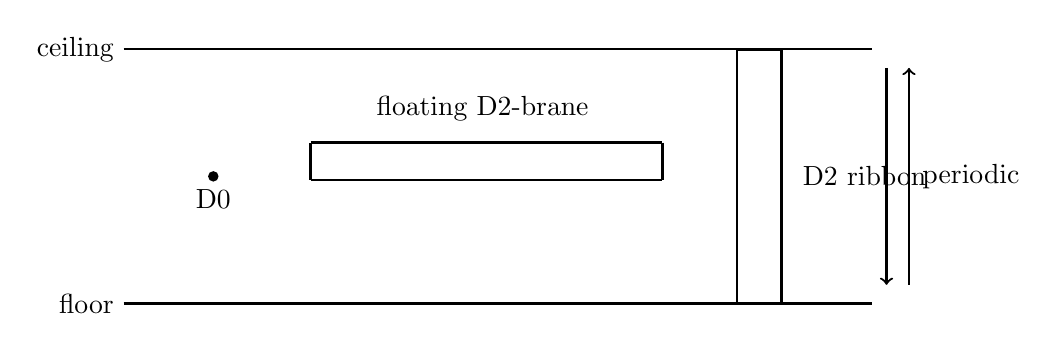
\begin{tikzpicture}[scale=0.95]
\draw[line width=0.9pt] (-5,1.7) -- (5,1.7);
\draw[line width=0.9pt] (-5,-1.7) -- (5,-1.7);

\node[left] at (-5,1.7) {ceiling};
\node[left] at (-5,-1.7) {floor};

\draw[->,line width=0.8pt] (5.2,1.45) -- (5.2,-1.45);
\draw[->,line width=0.8pt] (5.5,-1.45) -- (5.5,1.45);
\node[right] at (5.55,0) {periodic};

\draw[line width=1.0pt] (-2.5,0.45) -- (2.2,0.45);
\draw[line width=1.0pt] (-2.5,-0.05) -- (2.2,-0.05);
\draw[line width=1.0pt] (-2.5,0.45) -- (-2.5,-0.05);
\draw[line width=1.0pt] (2.2,0.45) -- (2.2,-0.05);
\node at (-0.2,0.9) {floating D2-brane};

\draw[line width=1.0pt] (3.2,-1.7) -- (3.8,-1.7);
\draw[line width=1.0pt] (3.2,1.7) -- (3.8,1.7);
\draw[line width=1.0pt] (3.2,-1.7) -- (3.2,1.7);
\draw[line width=1.0pt] (3.8,-1.7) -- (3.8,1.7);
\node[right] at (3.95,0) {D2 ribbon};

\fill (-3.8,0) circle (0.07);
\node[below] at (-3.8,-0.05) {D0};

\end{tikzpicture}
\caption{Transcript-based redraw of the sandwich compactification. The upper and lower boundaries are periodically identified; one D2-brane floats between them like a carpet, while another stretches from floor to ceiling and looks string-like when the compact direction is small.}
\end{figure}

The D2-branes supply the fate of the strings. There are two natural configurations in the lecture:
\begin{enumerate}
\item A membrane floating between floor and ceiling, like a carpet suspended in the peanut butter.
\item A ribbon stretching from floor to ceiling and extended along a visible direction.
\end{enumerate}
When the compact thickness is very small, the second object looks effectively one-dimensional. That is the string seen by low-energy observers. But as the compact direction grows, the same object becomes visibly membrane-like, acquires more material in the vertical direction, and becomes heavy.

\paragraph{Schematic evolution.}
\begin{enumerate}
\item Begin with a very thin compact direction, so the floor-to-ceiling ribbon looks like a string.
\item Increase \(g\), and the compact thickness grows.
\item D0-branes lighten and are reinterpreted as ordinary gravitons in the higher-dimensional theory.
\item The ribbon-like D2 object becomes less string-like and more membrane-like.
\item The correct strong-coupling language is therefore not another ten-dimensional string theory, but an effectively eleven-dimensional geometric theory.
\end{enumerate}

\section{D3-Branes and the Geometric Reinterpretation of Electric--Magnetic Duality}

After the break the lecture does not repeat the earlier arguments; it weaves them together. The first new idea is to use a D3-brane as a worldvolume on which ordinary-looking particle physics can occur.

\subsection{A D3-brane worldvolume}

A D3-brane has three spatial dimensions and, to an observer bound to it, looks like ordinary space. Fundamental strings can end on it, and so can D-strings. To the worldvolume observer, the endpoint of such a string is just a particle. The crucial point is that the two kinds of endpoints are not the same particle.

\begin{figure}[h]
\centering
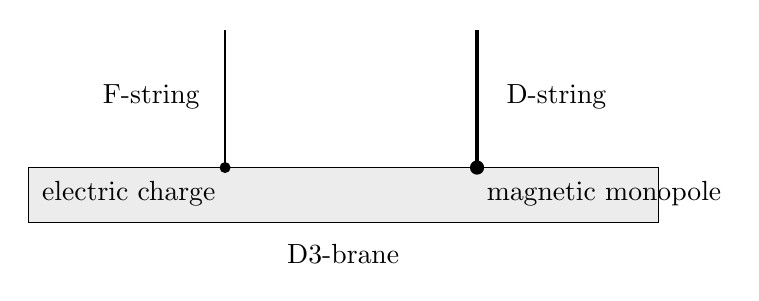
\begin{tikzpicture}[scale=1.0]
\draw[fill=gray!15] (-4,-0.35) rectangle (4,0.35);
\node at (0,-0.75) {D3-brane};

\draw[line width=0.9pt] (-1.5,2.1) -- (-1.5,0.35);
\fill (-1.5,0.35) circle (0.07);
\node[left] at (-1.7,1.25) {F-string};
\node[below left] at (-1.5,0.3) {electric charge};

\draw[line width=1.5pt] (1.7,2.1) -- (1.7,0.35);
\fill (1.7,0.35) circle (0.09);
\node[right] at (1.95,1.25) {D-string};
\node[below right] at (1.7,0.3) {magnetic monopole};
\end{tikzpicture}
\caption{Transcript-based redraw of the D3-brane worldvolume interpretation. An F-string endpoint appears as an electrically charged particle; a D-string endpoint appears as a magnetic monopole.}
\end{figure}

This is the lecture's payoff for the earlier analogies. The F-string/D-string duality is not merely analogous to electric--magnetic duality in field theory; on a D3-brane it becomes a concrete realization of it.

\subsection{Two compact directions and an asymmetric geometry}

Susskind then returns to the higher-dimensional geometric picture and compactifies not one but two directions. Since only three dimensions can be drawn on the board, the picture is necessarily schematic: one visible large direction stands in for many large dimensions, while two small directions are compact. He explicitly chooses an asymmetric case, because the asymmetry makes the comparison between light and heavy wrapped objects visible.

\begin{figure}[h]
\centering

\includegraphics[width=0.78\textwidth]{lecture_01_figure_03.png}

\vspace{1em}

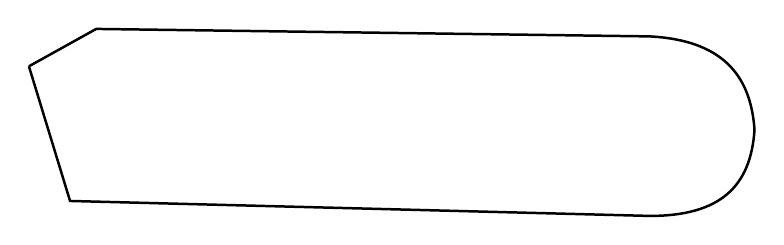
\begin{tikzpicture}[scale=0.95]
\draw[line width=0.9pt]
(-5,0.85) -- (-4.1,1.35) -- (3.3,1.25)
.. controls (4.25,1.20) and (4.65,0.75) .. (4.7,0.00)
.. controls (4.65,-0.75) and (4.25,-1.15) .. (3.3,-1.15)
-- (-4.45,-0.95) -- (-5,0.85);
\end{tikzpicture}
\caption{The asymmetric profile used to emphasize that the two compact directions are not equal. The screenshot is kept because the lecture's rhetoric here is strongly visual; the redraw regularizes only the large-scale shape.}
\end{figure}

The geometric content of the asymmetry is that a membrane wrapped one way around the compact directions becomes one effective string, while a membrane wrapped the other way becomes another effective string. Because one compact direction is shorter than the other, the two wrapped objects do not have the same effective weight. The lecture does not write a tension formula here, so we keep the statement qualitative: the wrapped object that uses more compact material is heavier.

Susskind then says explicitly that the earlier coupling parameter can be reinterpreted geometrically. The symbol \(\alpha\) is reused, but now it no longer denotes the QED fine-structure constant. It denotes an aspect ratio:
\begin{equation}
\alpha \sim \frac{R_1}{R_2},
\end{equation}
where \(R_1\) and \(R_2\) are clean editorial names for the two compactification scales. The lecture's physical point is that squeezing one direction while stretching the other interchanges which wrapped object is lighter. In that sense the geometry itself performs the weak--strong exchange.

\begin{figure}[h]
\centering

\includegraphics[width=0.78\textwidth]{lecture_01_figure_04.png}

\vspace{1em}

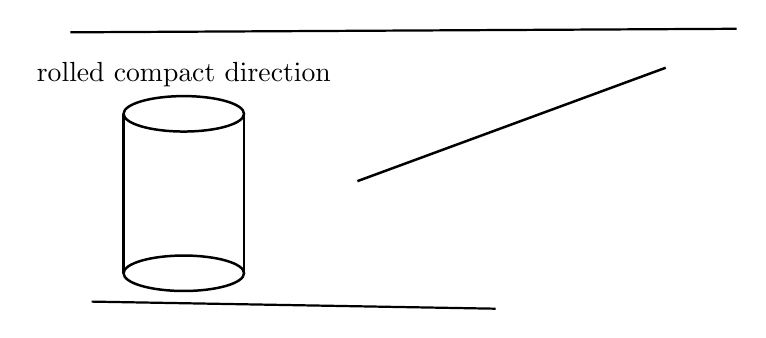
\begin{tikzpicture}[scale=0.9]
\draw[line width=0.9pt] (-3.6,0.9) ellipse (0.85 and 0.25);
\draw[line width=0.9pt] (-4.45,0.9) -- (-4.45,-1.35);
\draw[line width=0.9pt] (-2.75,0.9) -- (-2.75,-1.35);
\draw[line width=0.9pt] (-3.6,-1.35) ellipse (0.85 and 0.25);

\draw[line width=0.8pt] (-5.2,2.05) -- (4.2,2.10);
\draw[line width=0.8pt] (-4.9,-1.75) -- (0.8,-1.85);
\draw[line width=0.9pt] (-1.15,-0.05) -- (3.2,1.55);

\node at (-3.6,1.45) {rolled compact direction};
\end{tikzpicture}
\caption{Susskind's ``geometrical picture.'' The screenshot documents the board state at the moment he calls it geometric; the redraw keeps the cylinder-like compact direction, the long upper contour, and the slanted continuation without pretending to resolve every hidden chalk mark.}
\end{figure}

One should emphasize the lecture's caution here. This geometry is illuminating, but it is not supposed to solve every earlier question at once. In particular, it does not by itself display in an obvious way how a D-brane can look, under sufficiently hard probing, like a collection of F-strings. Susskind says exactly that: the geometric picture is useful, but it does not yet make every part of the duality transparent.

\section{Idealization, Specially Symmetric Points, and the Landscape}

The lecture closes by stepping back from the elegant examples. These dualities are mathematically tight, but they are also examples drawn from highly symmetric, supersymmetric theories. Susskind's own comparison is to circular orbits: one studies them first because they are tractable, not because the real world is composed of perfect circles. The same warning applies here.

In the geometric picture, there are specially symmetric points. The cleanest idealized statement is that equal aspect ratio makes the two wrapped descriptions coincide:
\begin{equation}
R_1=R_2
\qquad \Longrightarrow \qquad
\text{the two effective string descriptions coincide.}
\end{equation}
The lecture then translates the same symmetry back into the earlier electric--magnetic language:
\begin{equation}
m_{\mathrm{monopole}} = m_e
\end{equation}
at such a specially symmetric point. Susskind immediately adds the important physical caveat: our world does not appear to live at such a point.

\begin{figure}[h]
\centering

\includegraphics[width=0.78\textwidth]{lecture_01_figure_06.png}

\vspace{1em}

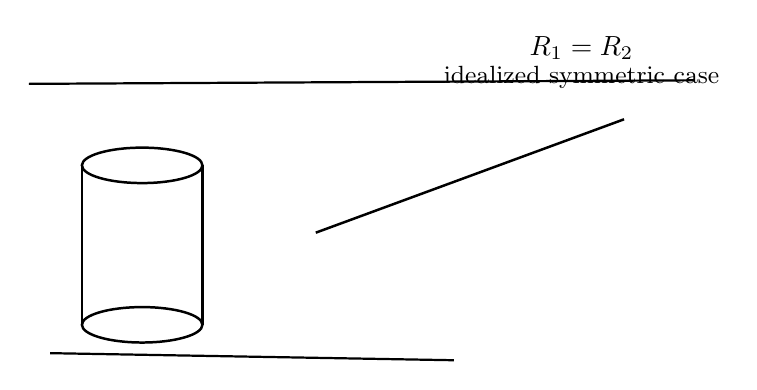
\begin{tikzpicture}[scale=0.9]
\draw[line width=0.9pt] (-3.6,0.9) ellipse (0.85 and 0.25);
\draw[line width=0.9pt] (-4.45,0.9) -- (-4.45,-1.35);
\draw[line width=0.9pt] (-2.75,0.9) -- (-2.75,-1.35);
\draw[line width=0.9pt] (-3.6,-1.35) ellipse (0.85 and 0.25);

\draw[line width=0.8pt] (-5.2,2.05) -- (4.2,2.10);
\draw[line width=0.8pt] (-4.9,-1.75) -- (0.8,-1.85);
\draw[line width=0.9pt] (-1.15,-0.05) -- (3.2,1.55);

\node at (2.6,2.55) {$R_1=R_2$};
\node at (2.6,2.15) {\small idealized symmetric case};
\end{tikzpicture}
\caption{Later board frame retained during the discussion of specially symmetric points. The equal-aspect annotation in the redraw is transcript-backed interpretation, not a direct transcription of visible chalk.}
\end{figure}

The next step in the lecture is combinatorial rather than geometric. String theory provides many kinds of building pieces: branes, fluxes, orbifolds, orientifolds, and complicated compact geometries. If a compact space has many cycles, and each cycle can be decorated in several ways, then the number of resulting vacua grows exponentially. Susskind's schematic estimate is
\begin{equation}
N_{\mathrm{vacua}} \sim 10^{500}.
\end{equation}
The lecture's mental model is simple: about \(500\) cycles, and roughly \(10\) choices per cycle, give
\begin{equation}
10\times 10\times \cdots \times 10 = 10^{500}
\end{equation}
with \(500\) factors. The DNA analogy says the same thing in a more familiar language:
\begin{equation}
N_{\mathrm{DNA}}(500)=4^{500}.
\end{equation}
The point is not the exact number. The point is that simple local rules can generate astronomically many globally complicated constructions.

That, in turn, suggests a different diagnosis of why particle physics is complicated. It may not be that the underlying rules are baroque. It may be that the rules are relatively simple, but the realized vacuum contains many moving parts. This is the lecture's final inversion of the original philosophical setup: complexity at low energies need not signal complicated microscopic laws. It may signal an enormous space of constructions.

The final coda of the lecture turns toward cosmology. A compact direction that is sufficiently large is observationally hard to distinguish from an infinite direction. Flatness by itself only places lower bounds on size; it does not prove infinity. At the same time, Susskind emphasizes that the mathematically idealized smooth spatial variation of couplings is not how our world seems to work. In the real world, if such variations exist at all, they appear to be restricted to discrete or step-like changes rather than smooth gradients.

\section{Summary}

The lecture begins with a simple philosophical expectation and systematically dismantles it. In \(1+1\)-dimensional bosonization, the same theory can be written in fermionic or bosonic variables, with the fermion reappearing as a kink. In QED, weak and strong coupling exchange the descriptive roles of electrons and magnetic monopoles. In string theory, F-strings and D-strings repeat the same pattern, and in the even-brane theory strong coupling goes further still: a compact direction expands, D0-branes become gravitons, and effective strings are reinterpreted as wrapped membranes. The final lesson is deliberately broader than any one example. Modern quantum field theory and string theory do not cleanly support a once-and-for-all distinction between houses and bricks. They support a network of descriptions, each efficient in its own regime, and a landscape of constructions whose generic output is complexity rather than simplicity.